\documentclass{article}
\usepackage{graphicx}
\usepackage{caption,rotating}
\usepackage{subfigure}
\begin{document}
\begin{figure}
\begin{turn}{90}
\begin{minipage}[c][\textwidth][c]{\textheight}
%\subfigure[Unfolded staple crimp type]{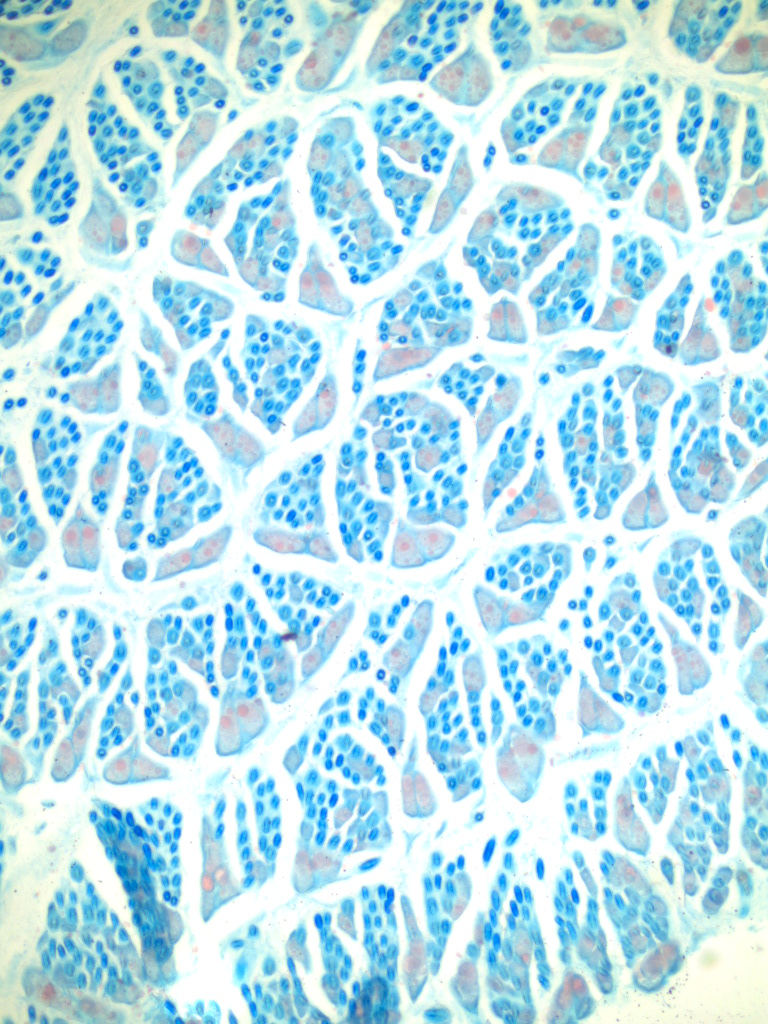
\includegraphics[width=.45\linewidth]{figskinhsunfrot.png}}\hfill
%\subfigure[Stretched staple crimp type]{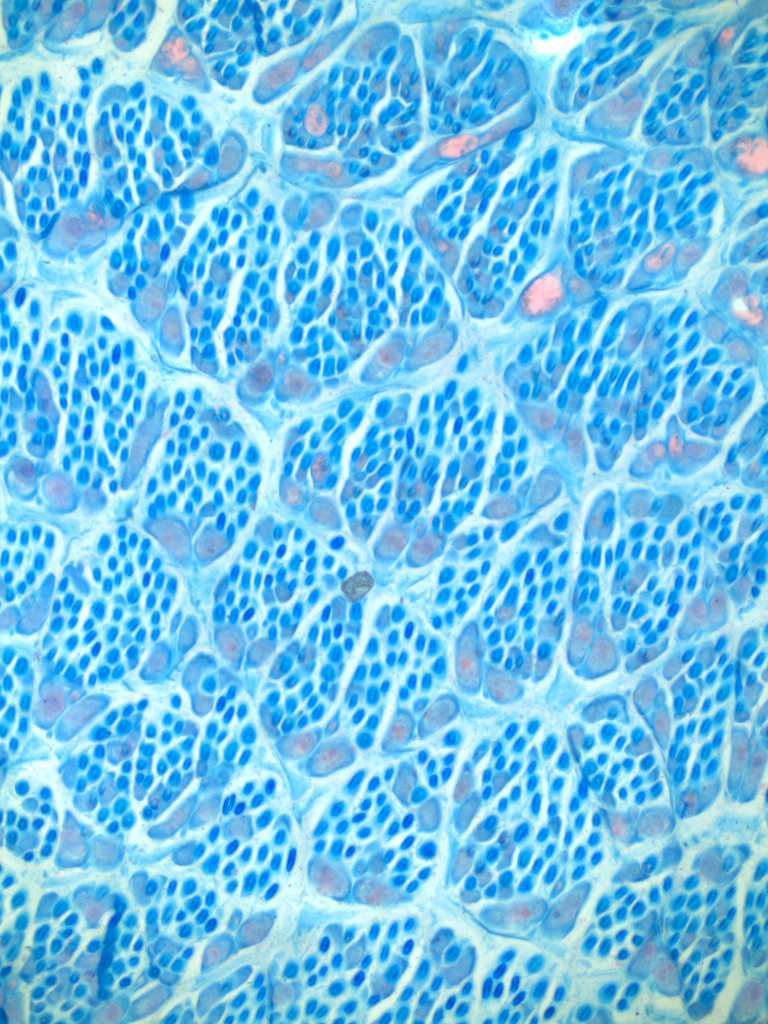
\includegraphics[width=.45\linewidth]{figskinhsstrrot.png}}
%\subfigure[Unfolded staple crimp type]{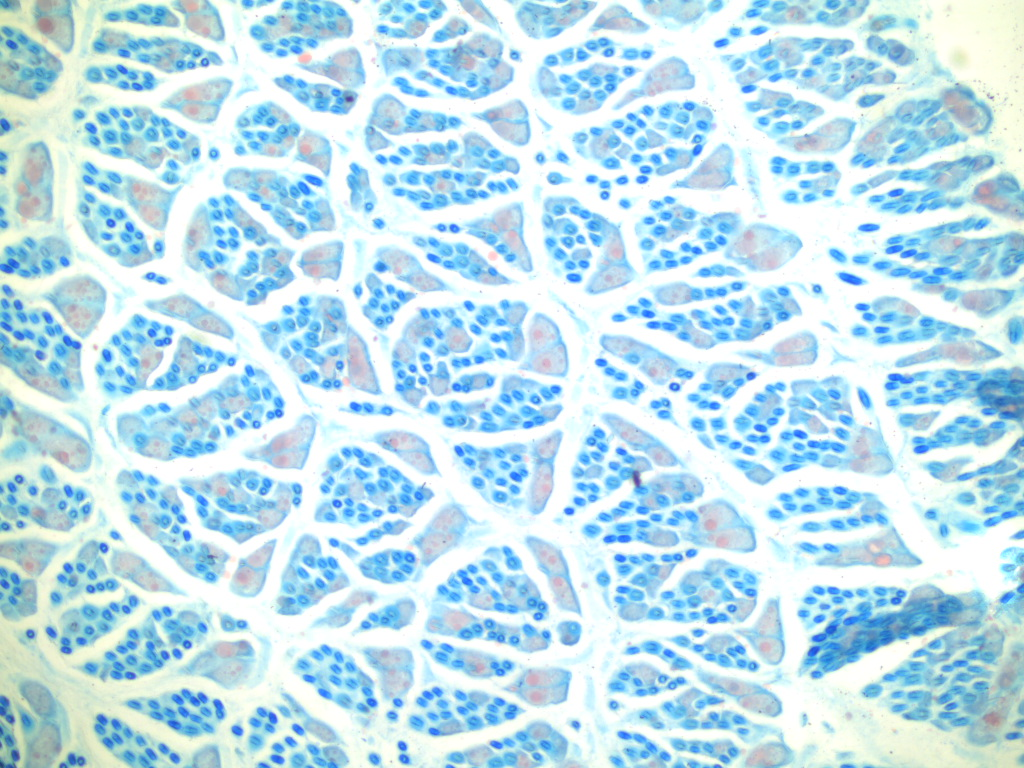
\includegraphics[height=.45\linewidth,angle=90]{figskinhsunf.png}}\hfill%
%\subfigure[Stretched staple crimp type]{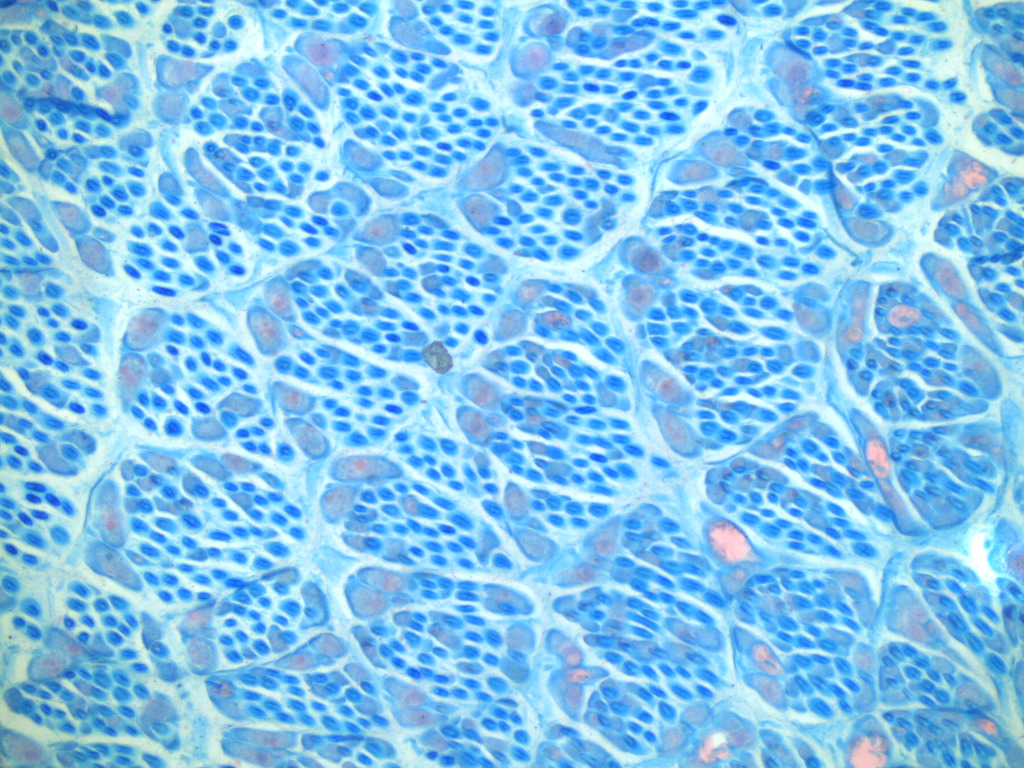
\includegraphics[height=.45\linewidth,angle=-90]{figskinhsstr.png}}
 \subfigure[Unfolded staple crimp type]{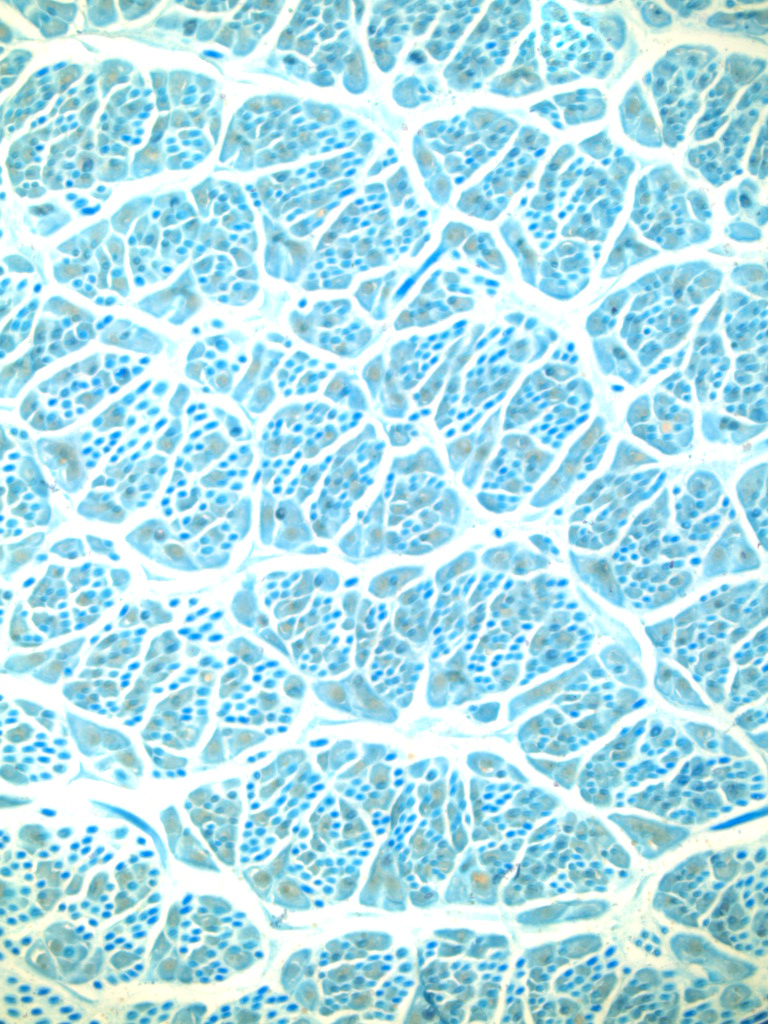
\includegraphics[scale=0.33]{studblunf.png}}\hfill
 \subfigure[Stretched staple crimp type]{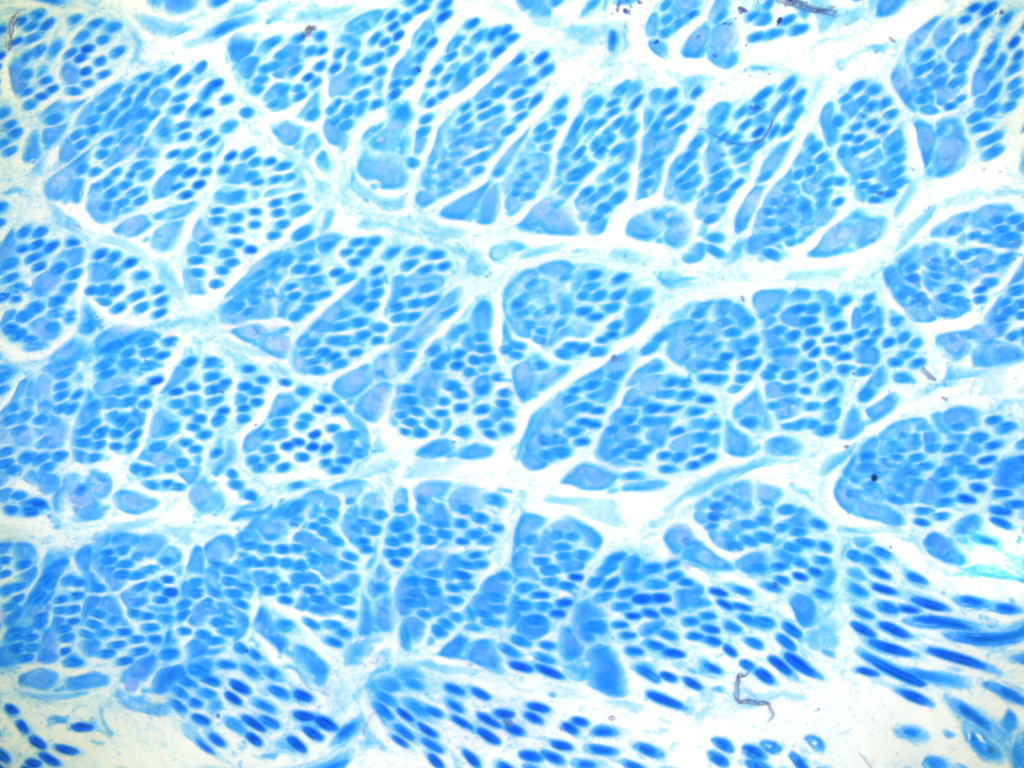
\includegraphics[scale=0.33]{JW2277.png}}
\caption{Horizontal skin sections from two Merino sheep, from the same flock, with unfolded helix crimp and stretched helix crimp. Note the  rows of follicle groups with appreciable connective tissue space between the rows in subfigure (a), and the absence of this feature in subfigure (b). The direction referred to as north-south is vertical and east-west is horizontal in both images. Stained with $0.5$\% Nile Blue Sulphate. Microscope magnification 25x. For printed or screen magnification see Appendix A }
\end{minipage}
\end{turn}
\end{figure}
\end{document}
